\documentclass[compress]{beamer}
\useoutertheme[footline=authorinstitutetitle]{miniframes}
\usecolortheme{whale}
\usecolortheme{orchid}
\useinnertheme{rounded}
\usepackage{xcolor}
\usepackage{listings}
\usepackage{placeins}
\lstset{ 
    language=Python, % choose the language of the code
    basicstyle=\footnotesize\color{black},
    keywordstyle=\color{black}\bfseries, % style for keywords
    commentstyle=\color{blue},
	stringstyle=\color{magenta},
    numbers=none, % where to put the line-numbers
    numberstyle=\tiny, % the size of the fonts that are used for the line-numbers     
    backgroundcolor=\color{white},
    showspaces=false, % show spaces adding particular underscores
    showstringspaces=false, % underline spaces within strings
    showtabs=false, % show tabs within strings adding particular underscores
    frame=single, % adds a frame around the code
    tabsize=2, % sets default tabsize to 2 spaces
    rulesepcolor=\color{gray},
    rulecolor=\color{black},
    captionpos=b, % sets the caption-position to bottom
    breaklines=true, % sets automatic line breaking
    breakatwhitespace=false, 
}

\setbeamerfont{block title}{size={}}

\def\raccoon{
\makebox[\linewidth][c]{\includegraphics[width=70pt]{/home/proycon/Pictures/Local/raccoon.pdf}\FloatBarrier}
}
\def\smallraccoon{
\makebox[\linewidth][c]{\includegraphics[width=30pt]{/home/proycon/Pictures/Local/raccoon.pdf}\FloatBarrier}
}



\title{FoLiA - Current state of affairs}
\author{Maarten van Gompel \\ \emph{Radboud University Nijmegen}}
\date{23 November 2012}
\usepackage{graphicx}


\begin{document}


\begin{frame}{FoLiA: Format for Linguistic Annotation}
	\begin{center}
		\Huge \textbf{FoLiA: Format for Linguistic Annotation} \\
		\large{Current state of affairs}
        
\includegraphics[width=25.0mm]{../../FoLiA-gh-pages/style/icon.png}
	\end{center}
\end{frame}


\section{Theoretical Background}
\subsection{Characteristics}

\begin{frame}

	\begin{block}{Intended Applications}
		\begin{itemize}
			\item as a corpus \textbf{storage} format
			\item as a language resource \textbf{exchange} format 
		\end{itemize}				
	\end{block}

	\begin{block}{FoLiA Characteristics}
		\footnotesize
		\begin{itemize}
			\item \textbf{Uniform} setup -- Consistent and uniform paradigm unifying various kinds of annotation. Not commited to any label set.
			\item \textbf{Extensible \& Flexible} -- Easy to extend
			\item \textbf{Expressive} -- Verbose expression of annotations, their annotators, timestamps, etc... Moreover, support for \emph{alternative} annotations. 
			\item \textbf{Formalised} -- Validation on shallow (structural) or deep level. The latter validates the label set and allows for links with for data category registries (e.g. ISOcat).			
			\item \textbf{Practical} -- Bottom-up development alongside libraries, various applications, different projects.
		\end{itemize}				
	\end{block}

\end{frame}

\subsection{Paradigm}

\begin{frame}
        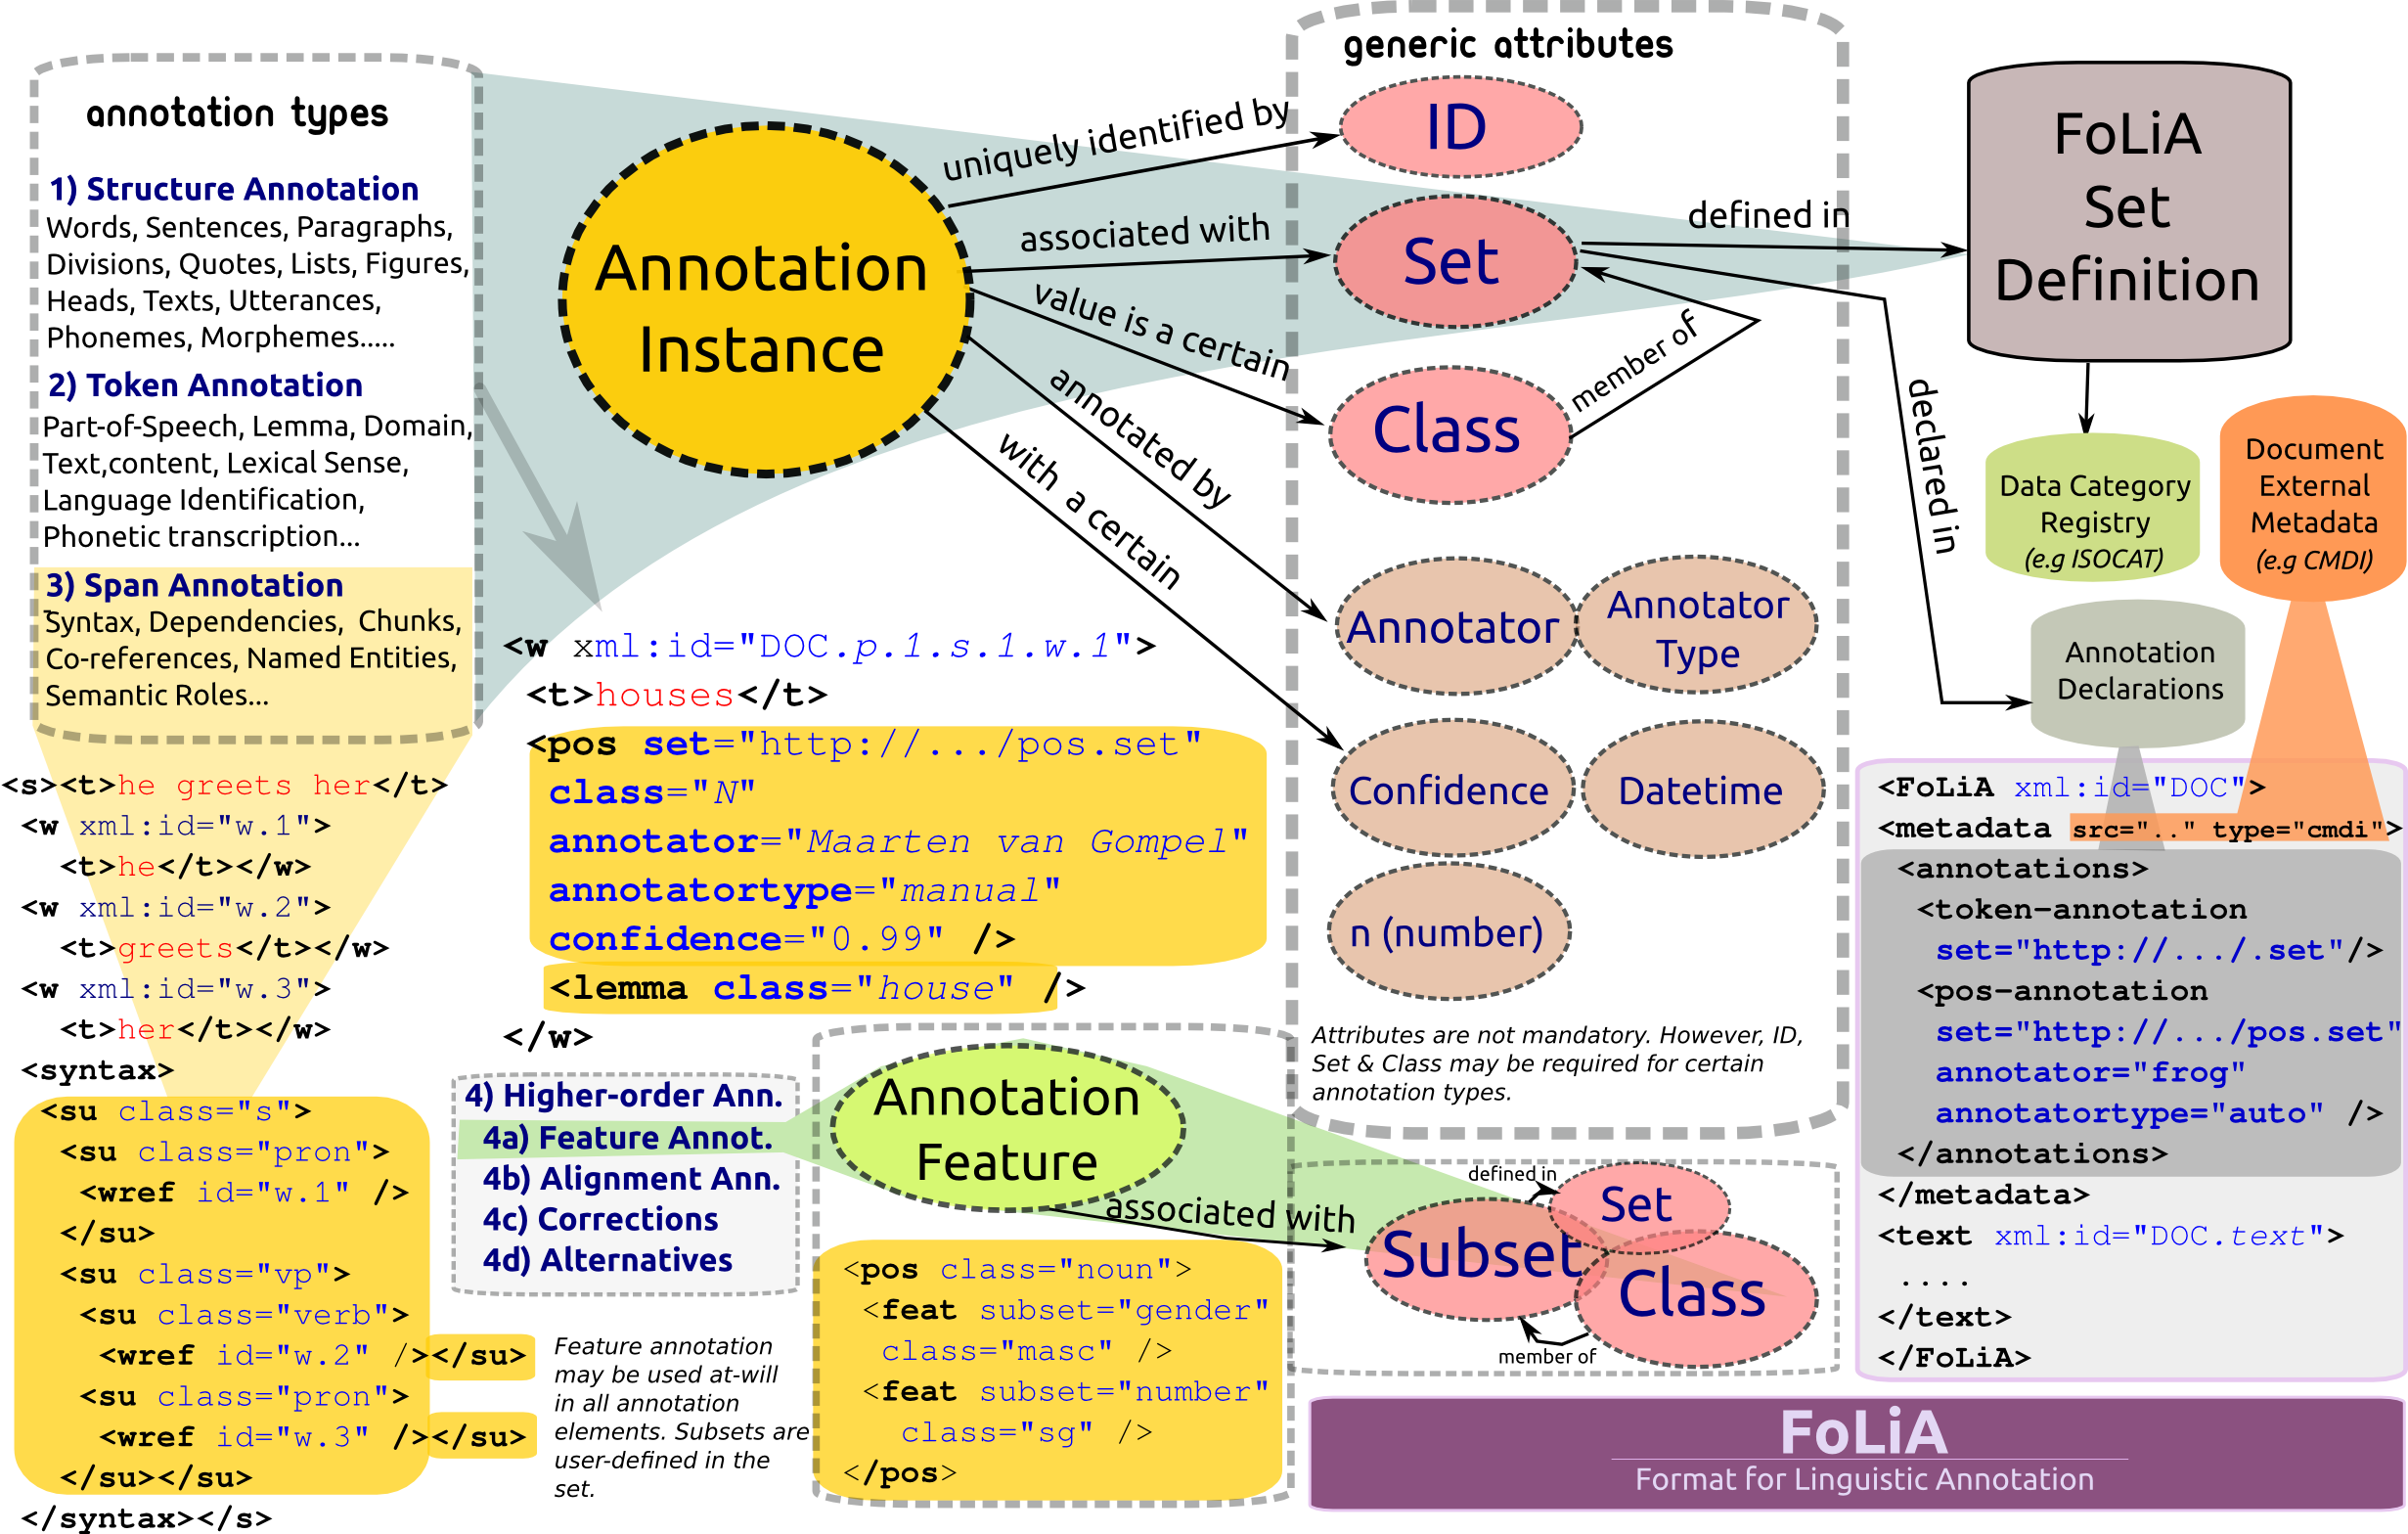
\includegraphics[width=115.0mm]{folia_paradigm.png}
\end{frame}


\begin{frame}
        \includegraphics[width=115.0mm]{folia_paradigm_p1.png}
\end{frame}


\begin{frame}
        \includegraphics[width=115.0mm]{folia_paradigm_p2.png}
\end{frame}

\begin{frame}
        \includegraphics[width=115.0mm]{folia_paradigm_p3.png}
\end{frame}

\begin{frame}
        \includegraphics[width=115.0mm]{folia_paradigm_p4.png}
\end{frame}

\begin{frame}
        \includegraphics[width=115.0mm]{folia_paradigm_p5.png}
\end{frame}

\begin{frame}
        \includegraphics[width=115.0mm]{folia_paradigm_p6.png}
\end{frame}

\begin{frame}
        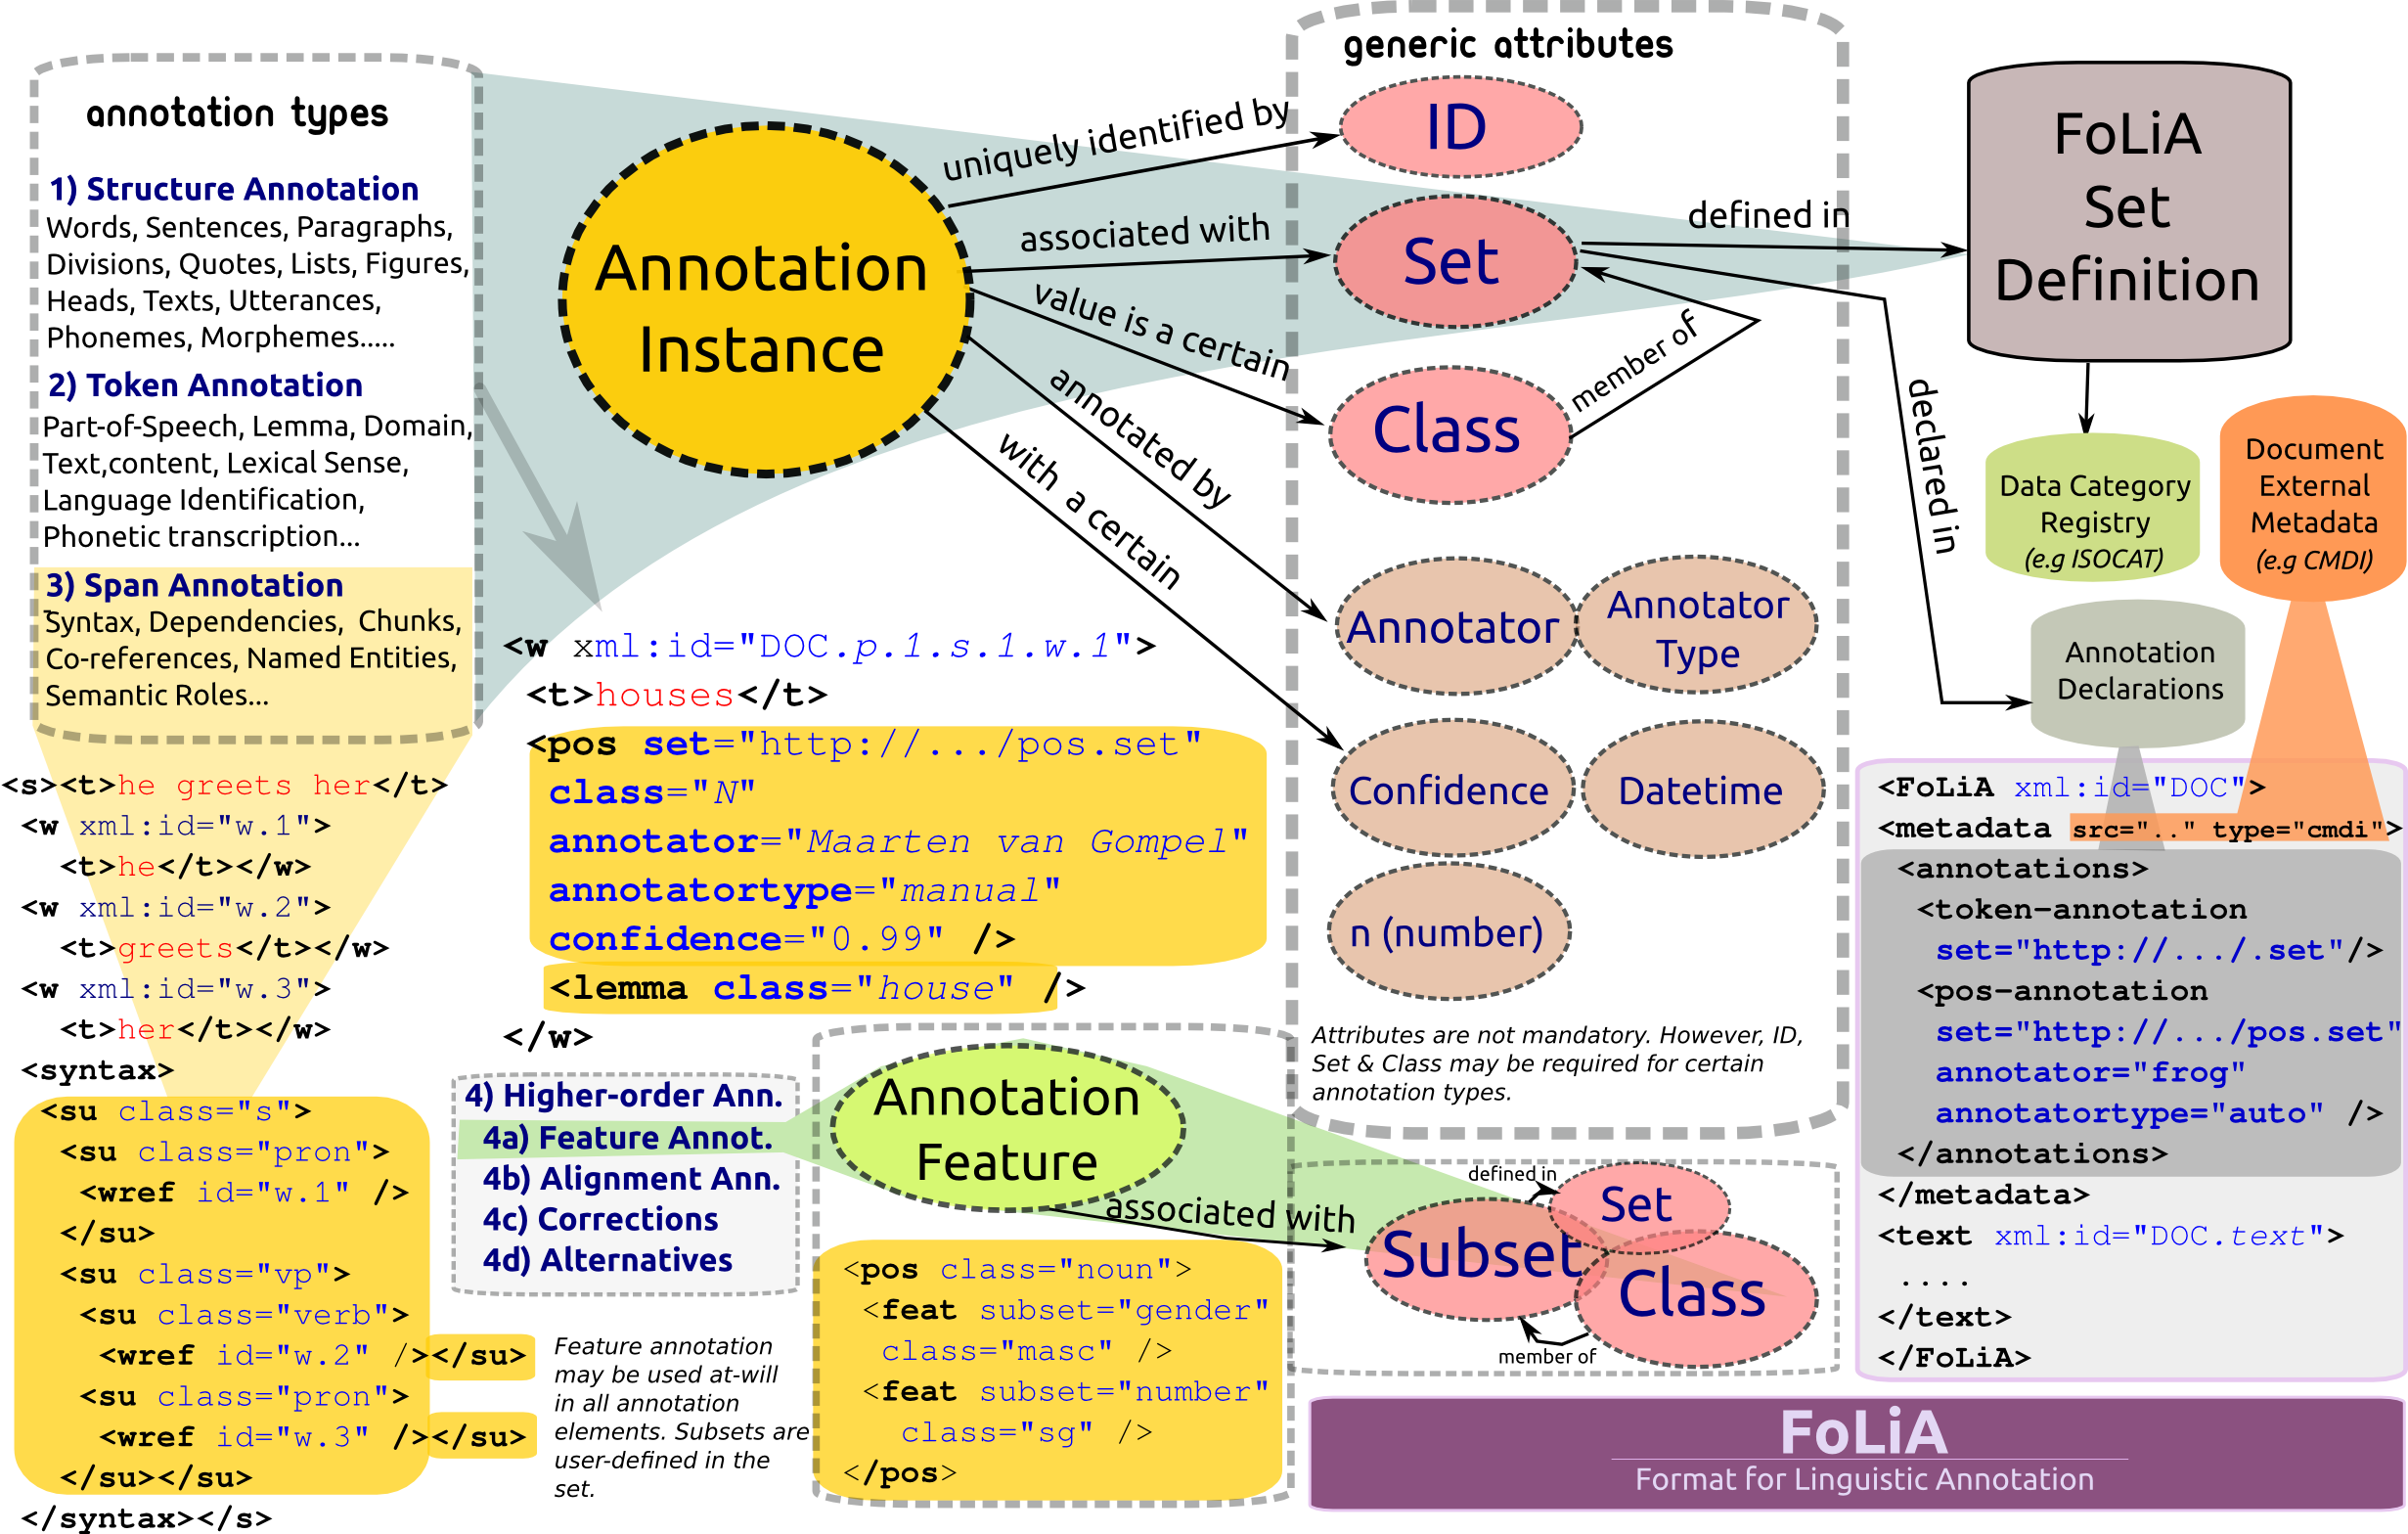
\includegraphics[width=115.0mm]{folia_paradigm.png}
\end{frame}


\section{Practice}
\subsection{Dissemination}

\subsection{Tools}

\begin{frame}
	\begin{block}{Tools for working with FoLiA}
		\begin{itemize}
			\item Standard \textbf{XML} facilities: XSLT, XPath
			\item \textbf{Python} library: pynlpl.formats.folia
			\item \textbf{C++} library: libfolia \emph{(Ko van der Sloot)}
		\end{itemize}
	\end{block}
	
	\begin{block}{FoliaTools}
		\textbf{Installation}: \texttt{ \$ easy\_install folia}
		\begin{itemize}
			\item \textbf{Converters}: folia2dcoi, dcoi2folia, folia2html, folia2columns, alpino2folia
			\item \textbf{Validator}: foliavalidator
			\item \textbf{Simple search tool}: foliaquery
			\item \textbf{Other}: foliamerge, foliafreqlist
		\end{itemize}
	\end{block}
\end{frame}

\subsection{Applications}

\begin{frame}
	\begin{block}{Applications using FoLiA}
		\begin{itemize}
			\item \textbf{Frog} -- tagger/lemmatisation/parser suite: FoLiA input \& output
			\item \textbf{ucto} -- tokeniser: FoLiA input and output
			\item \textbf{Valkuil.net} -- Dutch spelling checker
			\item \textbf{Fowlt.net} -- English spelling checker
			\item \textbf{Ticcl} -- Spelling normalisation
		\end{itemize}
	\end{block}

	\begin{block}{Corpora delivered in FoLiA}
		\begin{itemize}
			\item SoNaR \emph{(STEVIN)}, DutchSemCor \emph{(NWO)}, VU-DNC \emph{(CLARIN)}, Basilex \emph{(NWO)}
		\end{itemize}
	\end{block}		
\end{frame}
	

\subsection{Working with FoLiA from Python}

\begin{frame}[fragile]
\footnotesize
\begin{lstlisting}[language=python]
from pynlpl.formats import folia

#Load FoLiA document
doc = folia.Document(file='/path/to/folia_doc.xml')

#grab a specific sentence from the index
sentence = doc['folia_doc.s.1']

#print words in sentence along with PoS and lemma
for word in sentence.words():
    print word.text()  + ", " + word.pos() + ", " + word.lemma()	

#add PoS Annotation to a specific word
word = doc['folia_doc.s.1.w.5']
word.append( folia.PosAnnotation, cls="N",
  set="http://some/url/cgn.set")

doc.save() #Save edited document
\end{lstlisting}
\end{frame}


\subsection{Working with FoLiA: visualisation}

\begin{frame}[fragile]
   \includegraphics[width=110.0mm]{visexample.png}
\end{frame}



\subsection{Current state}

\begin{frame}
	\begin{block}{Recent developments}
	  \begin{itemize}
		\item Co-reference resolution
		\item Semantic roles
		\item Improvements in morphological annotation
		\item Speech annotation: first proposal
	  \end{itemize}
	\end{block}

	\begin{block}{Work in progress for the future}
	  \begin{itemize}
		\item Speech annotation, phonemes
		\item FoLiA Set Definitions and deep validation
		\item More tools and applications
	  \end{itemize}
	\end{block}
\end{frame}


\section{The End}

\begin{frame}

\raccoon

\begin{center}

\textbf{New website:} \texttt{http://proycon.github.com/folia} \\ 
\textbf{Later today:} FoLiA demo session including Frog, ucto, Python library. \\

\medskip

\Large{Questions?}


\end{center}


\section{Extra}

\subsection{Trade-off}


\begin{frame}
	\begin{block}{Trade-off: Expressivity versus Computing Efficiency}		
		\begin{itemize}
    			\item FoLiA aims at expressivity rather than computing efficiency. 
			\begin{itemize}
				\item XML and FoLiA overhead: Not ideal for real-time or resource-constrained applications
				\item \textbf{Conversion} to less expressive, more efficient, formats.
			\end{itemize}			 
		\end{itemize}	
	\end{block}
\end{frame}


\begin{frame}[fragile]
\frametitle{Alternative Token Annotations}

Annotations of the same type, but different sets need \emph{not} be alternatives.

\begin{lstlisting}[language=xml]
<w xml:id="example.p.1.s.1.w.2">
    <t>luid</t>
    <pos set="brown" class="jj" />
    <pos set="cgn" class="adj" />
</w>                         
\end{lstlisting}        

There can be only one of the same set though, this is illegal and requires usage of alternatives instead:

\begin{lstlisting}[language=xml]
<w xml:id="example.p.1.s.1.w.2">
    <t>luid</t>
    <pos set="cgn" class="adj" />
    <pos set="cgn" class="adv" />
</w>                         
\end{lstlisting}   

\end{frame}


\begin{frame}[fragile]
\frametitle{Alternative Token Annotations}

Encodes mutually exclusive alternative annotations. Any annotations that are not alternatives are considered ``selected''.

\begin{lstlisting}[language=xml]
<w xml:id="example.p.1.s.1.w.2">
    <t>bank</t>
    <sense set="wordnet3.0" class="bank%1:17:01:"    
     annotator="Maarten van Gompel" annotatortype="manual" 
     confidence="0.8">
     <desc>sloping ground near water</desc></sense>
    <alt xml:id="example.p.1.s.1.w.2.alt.1">
     <sense set="wordnet3.0" class="bank%1:14:01:"
      annotator="WSDsystem" annotatortype="auto" 
      confidence="0.6">     
      <desc>financial institution</desc></sense> 
    </alt>
</w>                         
\end{lstlisting}        

\end{frame}

\begin{frame}[fragile]
\frametitle{Alternative Token Annotations}

All token annotations grouped as one alternative are considered dependent. Multiple alternatives are always independent:

\begin{lstlisting}[language=xml]
<w xml:id="example.p.1.s.1.w.2">
    <t>vlieg</t>
    <pos class="N" />
    <lemma class="vlieg" />
    <alt xml:id="example.p.1.s.1.w.2.alt.1">
        <pos class="V" />
        <lemma class="vliegen" />
    </alt>
</w>                         
\end{lstlisting}        

\end{frame}

\end{frame}








\end{document}
